\chapter{Discussion}  
\subsection{Simplified Test Cases}
With each of the schemes previously discussed, the method of evaluation consisted of an explicit curvature calculation of an exact VOF field followed by an oscillating droplet test case. Consistently, the exact curvature estimation was successful and the oscillating droplet problematic. The transition between the test cases began to seem like too great of a jump in complexity to have an intimate understanding of the progression of errors occurring. To gain a deeper understanding of the source of failure, it seemed necessary to have more simplified test cases with which to study the method. To this end, four simplified test cases were developed which we hoped would expose the limitations of the schemes.

\subsubsection{Sine Wave Test Case}
A sinusoidal interface was constructed as seen in Figure~\ref{fig:sine}. The test case was created specifically to test several key aspects of the method. First, by modifying the geometry of the sinusoid its possible to test internal and external face fluxes independently or jointly. Secondly, because the interface is highly symmetric, variation in velocity and curvature values across the domain helps to highlight deficiencies in boundary conditions as well as inter-cell transport schemes. The goal of this test case is for the fine grid scheme to force a collapse of the interface so that a final curvature of zero is achieved.  
 \begin{figure}
 	\centering
 	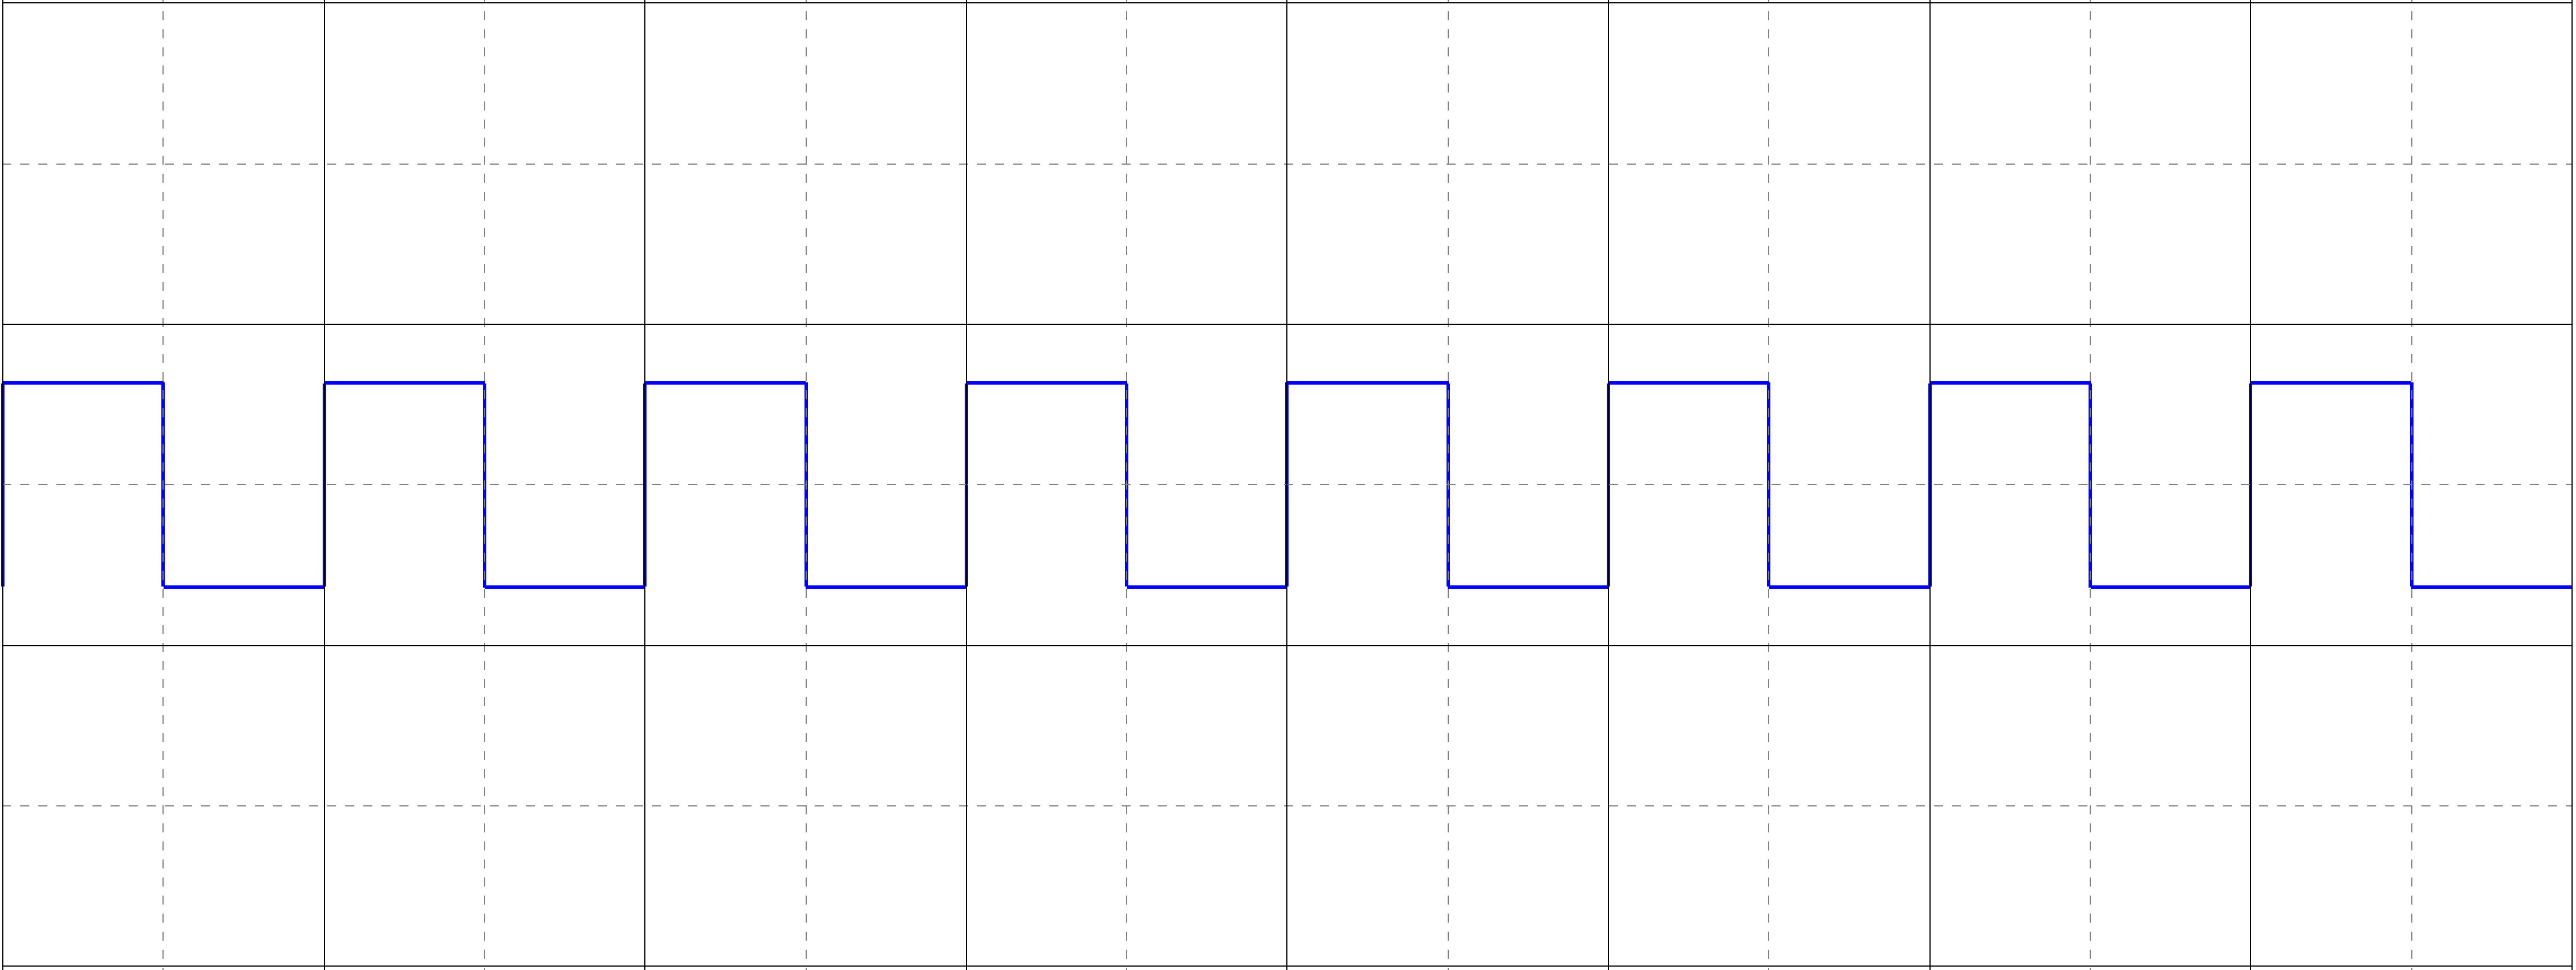
\includegraphics[width=0.5\textwidth]{figs/sine}
 	\caption{fix figure}
 	\label{fig:sine}
 \end{figure}

\subsubsection{Interfacial Protrusion Test Case}
The test cases shown in Figures~\ref{fig:0},~\ref{fig:90}, \&~\ref{fig:45} are all of a simple linear interface at various orientations. At the center of each domain, a protrusion was placed on the interface. The aim of this test case was to recreate specific, isolated, scenarios to see if the fine grid method could accomplish collapsing the interface to a line and obtain a zero curvature across the domain. The protrusion on each interface was built to be approximately one cell width in both height and width. 

\begin{figure}[htbp]
	\centering
	\begin{minipage}{0.3\textwidth}
		\fbox{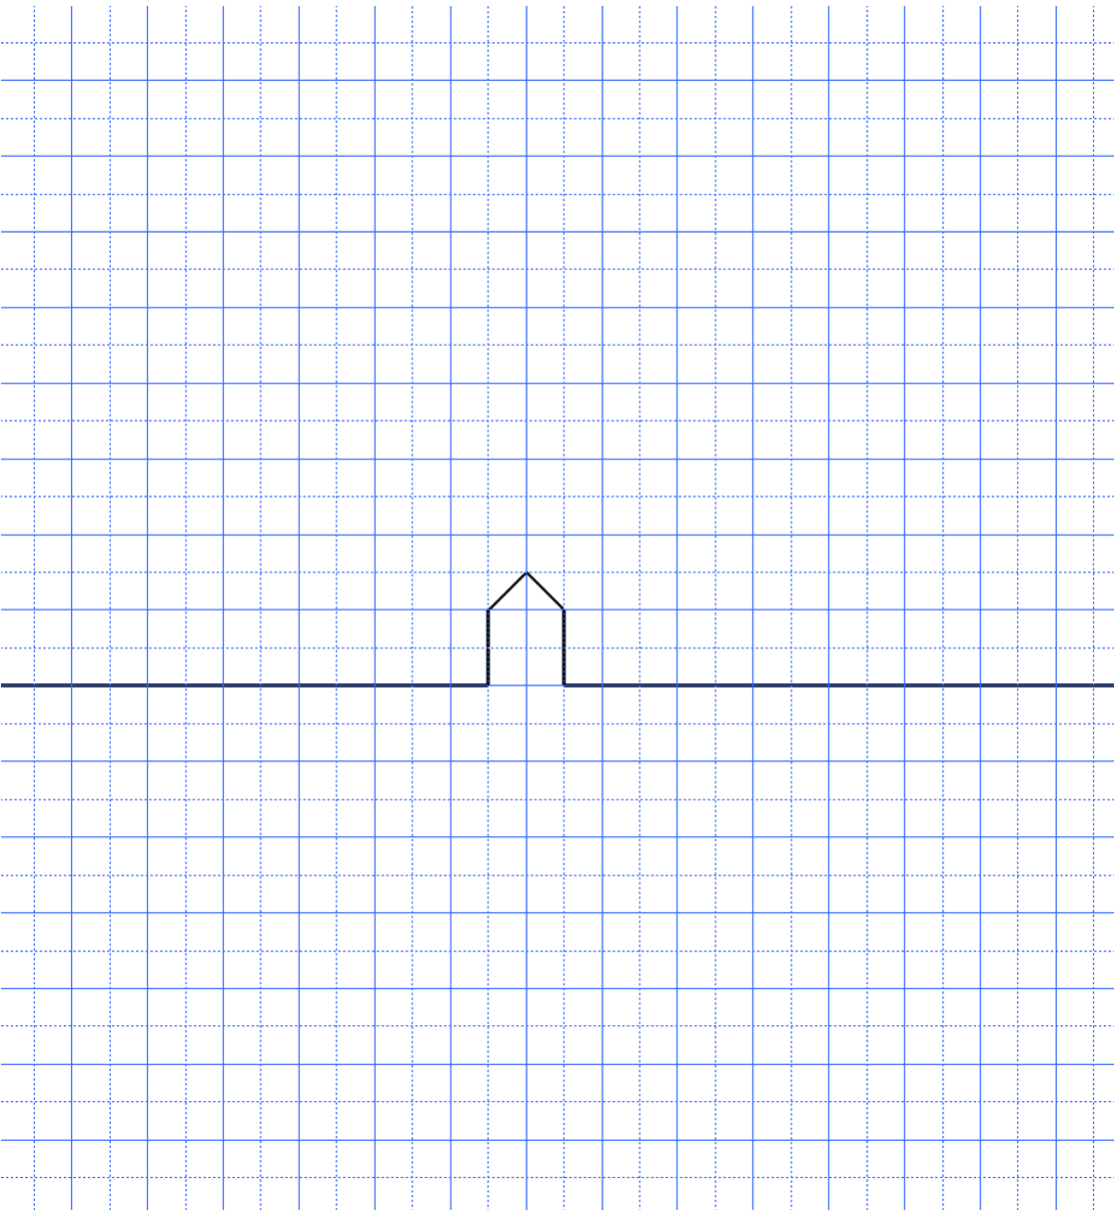
\includegraphics[width=0.95\linewidth]{figs/0}}
		\caption{fix figure}
		\label{fig:0}
	\end{minipage}%
	\begin{minipage}{0.3\textwidth}
		\fbox{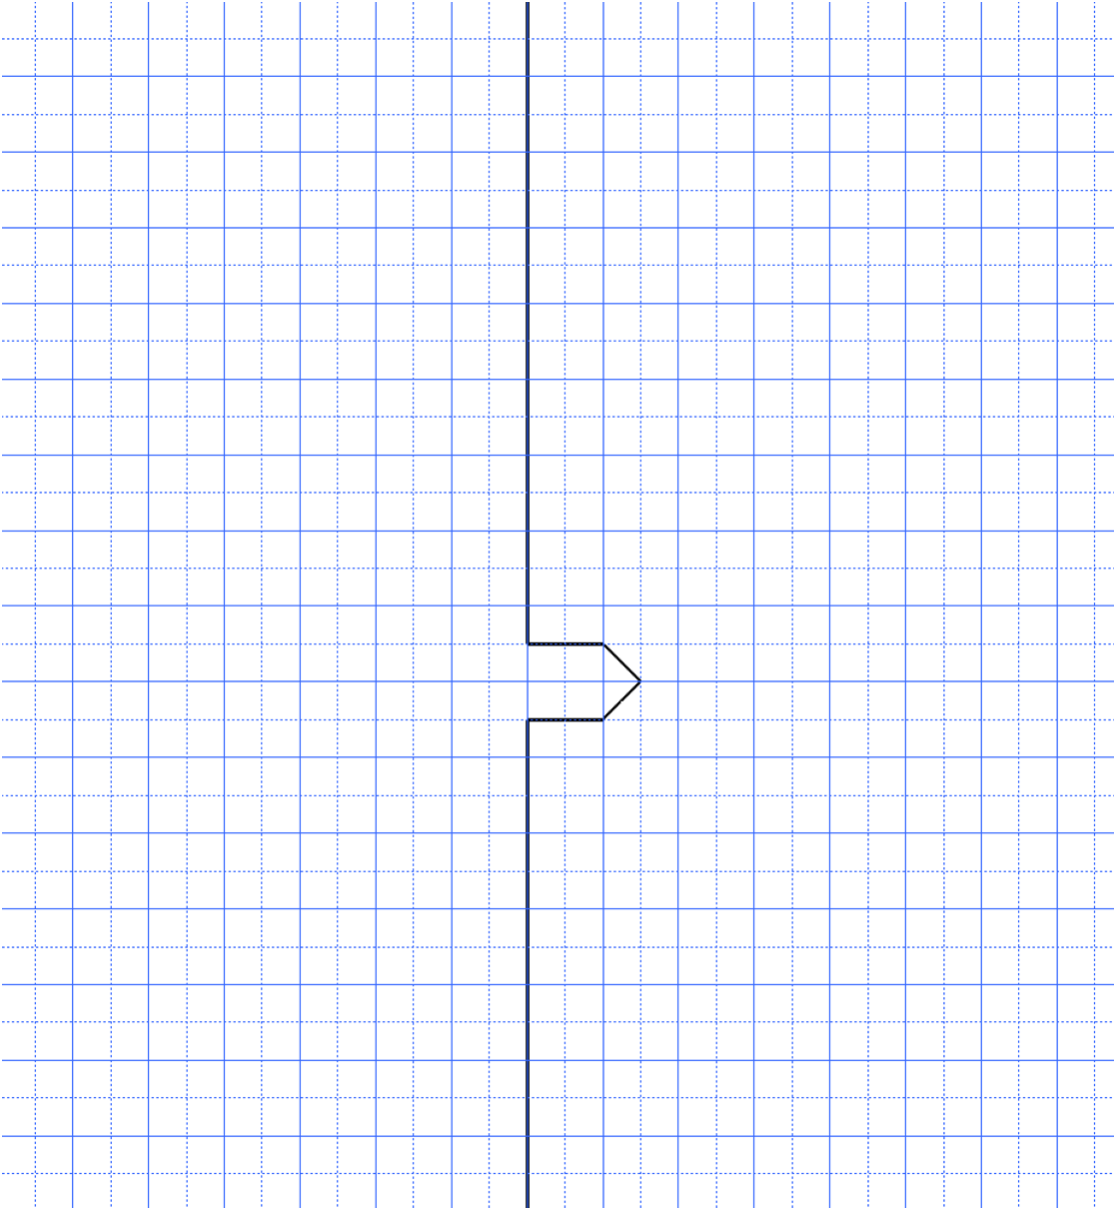
\includegraphics[width=0.95\linewidth]{figs/90}}
		\caption{fix figure}
		\label{fig:90}
	\end{minipage}
	\begin{minipage}{0.3\textwidth}
		\fbox{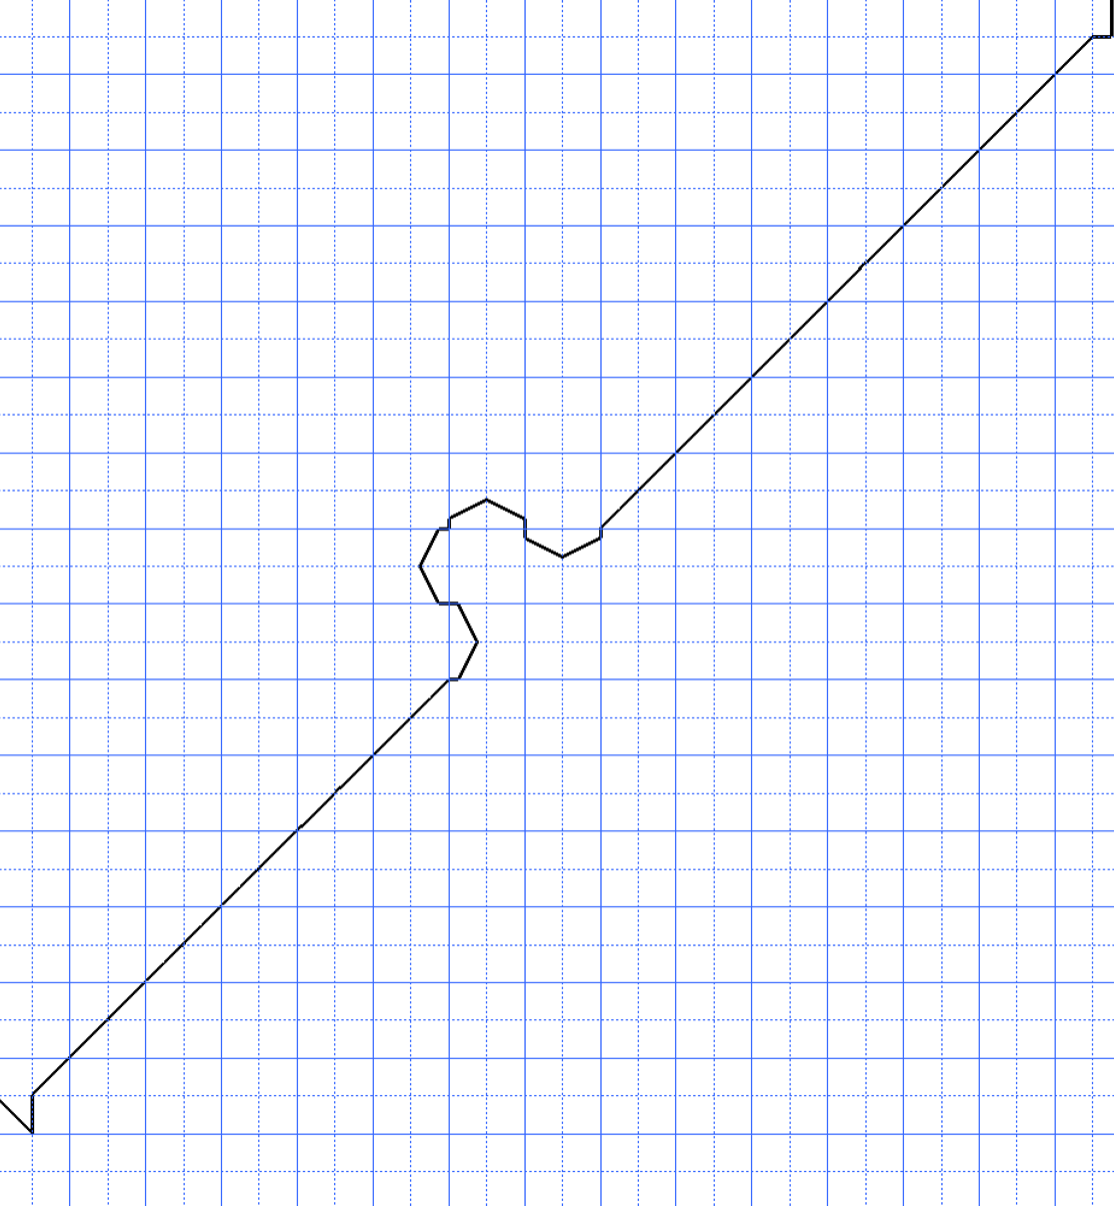
\includegraphics[width=0.95\linewidth]{figs/45}}
		\caption{fix figure}
		\label{fig:45}
	\end{minipage}
\end{figure}

\begin{figure}
	\centering
	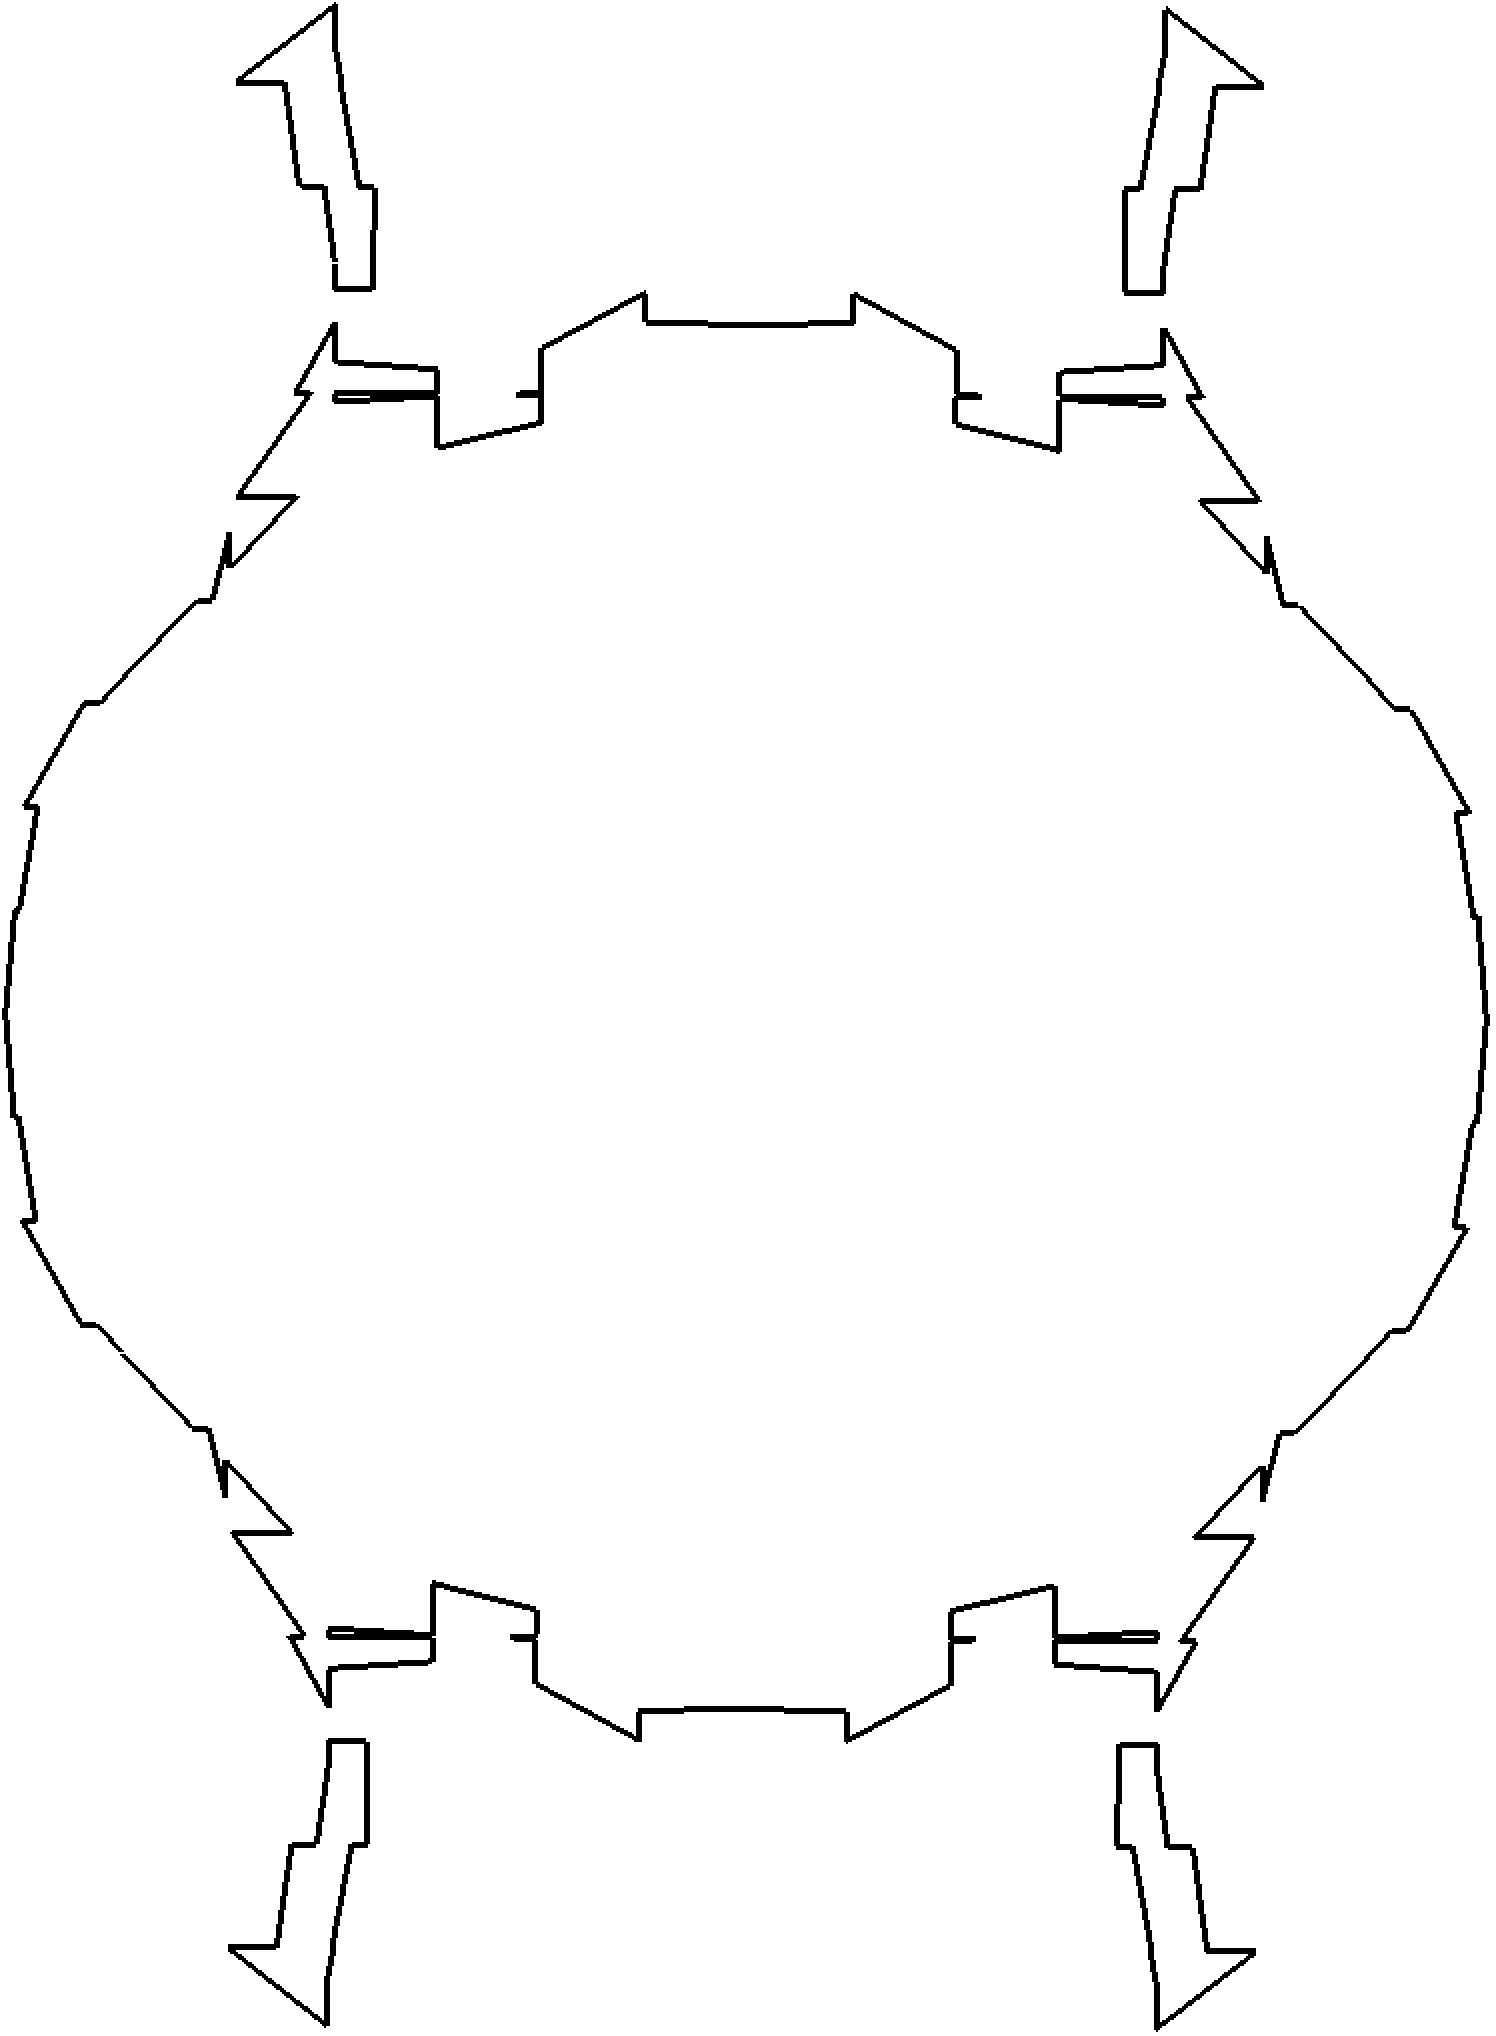
\includegraphics[width=0.5\textwidth]{figs/bad.png}
	\caption{fix figure}
	\label{fig:45s}
\end{figure}
For each of the above test cases, with the exception of the $45^{\circ}$ test case, the method was successful in collapsing the interface to a line. This was an interesting discovery and seemed to coincide with results seen in failing oscillating droplet test cases. During the oscillating droplet test, often nonphysical geometries would begin to appear at each of the quadrant regions of the droplet as shown in Figure~\ref{fig:45s}. This finding exposed a key limitation of the model. Well defined heights are not present in this case and cause problems for the height function method. When heights are not well defined, the approximation of derivatives is not accurate and results in nonphysical geometries.  

At the current state, the fine grid method can successfully predict curvature for a select set of geometries. No successful execution of three dimensional flows have been performed or analyzed. Rigorous investigation of the methods outlined above have left the researchers with several fundamental concerns and drawbacks of this method can be summarized as
\begin{enumerate}
	\item It is clear that this method, in all iterations, requires well defined heights for successful execution. However, achieving well defined heights may require mesh sizes which are unrealistic for direct numerical simulation. While there may possibly be ways to work around this issue, research thus far has focused on performing successful simulations with geometries that provide ideal mesh size ratios. Investigation into more complex schemes should only be attempted after this has been achieved.
	\item Incorporation of fine grid velocities seemed to have a positive impact on success of the system but required several modifications from the originally proposed method. The addition of a second pressure equation makes this method computationally expensive. So much so that simulation run time can increase by $40\%$. This increased expense contradicts original motivation of the investigation. Modification of the height function method was chosen as implementing the method is straightforward and the cost is low compared to more complex methods. To that point, while the fine grid height function is straightforward to implement, fine grid velocity incorporation and the subsequent incorporation of semi-lagrangian fluxes are not. 
	\item While little investigation has been done with three dimensional flow fields, accurate and realistic curvature becomes significantly harder to achieve as fitting is now done using planes instead of lines.
	\item To present, efforts have been considering a simulation which doesn't "blow up" to be a success. However, no efforts have gone into investigating the accuracy of this model. This is vital to understanding the merit of the method. 
\end{enumerate} 

%\begin{figure}
%\begin{tikzpicture}[scale=4.25]
%% Heights
%\draw [black, fill=cyan!20] plot [smooth ] coordinates {(0.25,0.3)(0.75,0.5)(1.25,0.1)(1.75,0.6)(2.25,0.3)(2.75,0.7)} -- (2.75,0) -- (0.25,0) -- cycle;
%\draw [fill] (1.5,0.36) circle [radius=0.05];
%\node [above ] at (1.5,0.45) {$\kappa$};
%\draw [arrows=->,line width=1.0] (0.25,0) -- (0.25,0.3);\node [below] at (0.25,0) {\scriptsize $h_{-3}$};
%\draw [arrows=->,line width=1.0] (0.75,0) -- (0.75,0.5);\node [below] at (0.75,0) {\scriptsize $h_{-2}$};
%\draw [arrows=->,line width=1.0] (1.25,0) -- (1.25,0.1);\node [below] at (1.25,0) {\scriptsize $h_{-1}$};
%\draw [arrows=->,line width=1.0] (1.75,0) -- (1.75,0.6);\node [below] at (1.75,0) {\scriptsize $h_{1}$};
%\draw [arrows=->,line width=1.0] (2.25,0) -- (2.25,0.3);\node [below] at (2.25,0) {\scriptsize $h_{2}$};
%\draw [arrows=->,line width=1.0] (2.75,0) -- (2.75,0.7);\node [below] at (2.75,0) {\scriptsize $h_{3}$};
%\end{tikzpicture}
%\caption{$5^{th}$ Order Fit of Heights}
%\label{fig:5thhts}
%\end{figure}

\subsection{Future Work}
DONT DO IT
%\section{Outline}
%\begin{Verbatim}[tabsize=4]
%	-We currently have a method that "kind of" works
%		*2D has been majority of testing
%	-We've learned that well defined heights are essential at all scales
%	-Drawbacks of this method:
%		*Well definied hts req mesh sizes that may be unrealistic for 
%		 multphase DNS sims
%		*Additional pressure eqn makes this method incredibly expensive 
%			-this is counter to our original motivation of cheap and easy
%			-To be fair, we're using Gauss Sidel and this leaves room 
%			 for improvement
%		*Moving to 3D becomes more complex as hts are now built with
%		 planes instead of PLIC's
%			-Further investigation needed to determine limitations
%		*Up until now oour metric of success has been "does the sim blow up?"
%			-if not we move on... but, no analysis has been done to test how 
%			  accurate the scheme is
%\end{Verbatim}